\chapter{视觉与大脑}\label{ch:g11:vision-and-brain}

脑卒中后，一名患者看世界清晰如常，只是所见
只有黑、白和灰。另一名患者能看到颜色和形状，
却看不到运动：汽车时而在这里，时而在那里，
中间似乎什么也没有；倒茶也无法完成，因为水流
似乎从不移动。第三名患者无法认出人脸，
包括镜子里自己的脸，尽管能逐一说出每一个
面部特征。他们的眼睛都没有损伤，各自失去的，
是大脑中负责把所见组装起来的那一部分。
本章追随视神经进入大脑，描绘视觉皮层如何处理
视网膜传来的信号，并说明这张地图并非一成不变：
它由经验构建，因学习而改变，还会受药物干扰。

\section{从视网膜到皮层}

\begin{proposition}[视觉通路]\label{prop:g11:vision-and-brain:pathway}
每条视神经的一百万根纤维向后延伸，
汇入\emph{视交叉}。在视交叉处，来自每只眼睛视网膜
鼻侧一半的纤维交叉到对侧，
而来自颞侧一半的纤维则留在同侧。
越过视交叉后，每条\emph{视束}因此携带
两眼视网膜左半部分的信号（右侧视束）或右半部分的信号
（左侧视束），也就是说，它承载的是视野一侧的全部所见。
视束在\emph{丘脑}中转接，并到达每个大脑半球后部的
\emph{初级视觉皮层}\index{视觉皮层}：左半球接收视野的右半部分，
右半球接收左半部分。
\end{proposition}
\begin{proof}[证据]
切断一条视神经会使一只眼睛失明；视束或一侧大脑
半球的视觉皮层受损，则两眼仍能工作，但两眼都会
对同一半视野失明，即与损伤相对的那一半。
手术中刺激清醒患者视觉皮层的一个点，
会使其在视野中某一固定位置看到闪光；
邻近的点产生邻近的闪光。由此可知，皮层保存着
一张视网膜的地图，
视野中心占据其中最大的部分。
\end{proof}

\begin{omfigure}
\begin{tikzpicture}[font=\small, >=Stealth, line cap=round]
  % top view: eyes at top, cortex at bottom
  \draw[thick, fill=omDef!8] (-2.2,4.2) circle (0.6); \draw[thick, fill=omDef!8] (2.2,4.2) circle (0.6);
  \node[anchor=south] at (-2.2,4.9) {左眼}; \node[anchor=south] at (2.2,4.9) {右眼};
  % visual field halves
  \node[omThm, anchor=east] at (-3.2,5.9) {左视野};
  \node[omMeth!60!black, anchor=west] at (3.2,5.9) {右视野};
  \draw[omThm, thick] (-4.4,5.6) -- (0,5.6); \draw[omMeth!60!black, thick] (0,5.6) -- (4.4,5.6);
  % fibres: left field falls on right halves of both retinas -> right hemisphere
  % from left eye: temporal half (left side of left eye) sees right field -> stays left; nasal half sees left field -> crosses
  \draw[thick, omMeth!60!black] (-2.7,3.7) -- (-2.7,1.6) -- (-1.2,0.3) -- (-1.2,-1.4);
  \draw[thick, omThm] (-1.7,3.7) -- (-1.7,1.6) -- (1.2,0.3) -- (1.2,-1.4);
  \draw[thick, omThm] (2.7,3.7) -- (2.7,1.6) -- (1.2,0.3);
  \draw[thick, omMeth!60!black] (1.7,3.7) -- (1.7,1.6) -- (-1.2,0.3);
  \fill (0,0.85) circle (2pt); \node[anchor=north] at (0,0.4) {视交叉};
  % thalamus relays
  \draw[thick, fill=gray!20] (-1.2,-0.4) ellipse (0.35 and 0.25); \draw[thick, fill=gray!20] (1.2,-0.4) ellipse (0.35 and 0.25);
  \node[anchor=east] at (-1.6,-0.4) {丘脑};
  % cortex
  \draw[thick, fill=omMeth!15] (-2.4,-2.6) rectangle (-0.2,-1.4); \draw[thick, fill=omThm!15] (0.2,-2.6) rectangle (2.4,-1.4);
  \node[align=center] at (-1.3,-2.0) {左侧视觉 \\皮层}; \node[align=center] at (1.3,-2.0) {右侧视觉 \\皮层};
  \node[anchor=north, align=center, font=\scriptsize] at (-1.3,-2.7) {接收右侧 \\视野};
  \node[anchor=north, align=center, font=\scriptsize] at (1.3,-2.7) {接收左侧 \\视野};
  \node[anchor=west, align=left, font=\scriptsize] at (3.0,2.6) {视神经：\\每只眼一条};
  \node[anchor=west, align=left, font=\scriptsize] at (3.0,0.0) {视束：\\每个半视野一条};
\end{tikzpicture}

{\small 从上方看到的视觉通路。来自视野左半部分（红色）的光
落在每个视网膜的右半部分上；这些纤维在视交叉处按需交叉，
汇入右侧视束，
并到达右侧视觉皮层。
每个半球借助双眼看到世界的对侧一半。}
\end{omfigure}

\begin{omfigure}
\begin{tikzpicture}
  \node[anchor=south west, inner sep=0] (img) at (0,0)
    {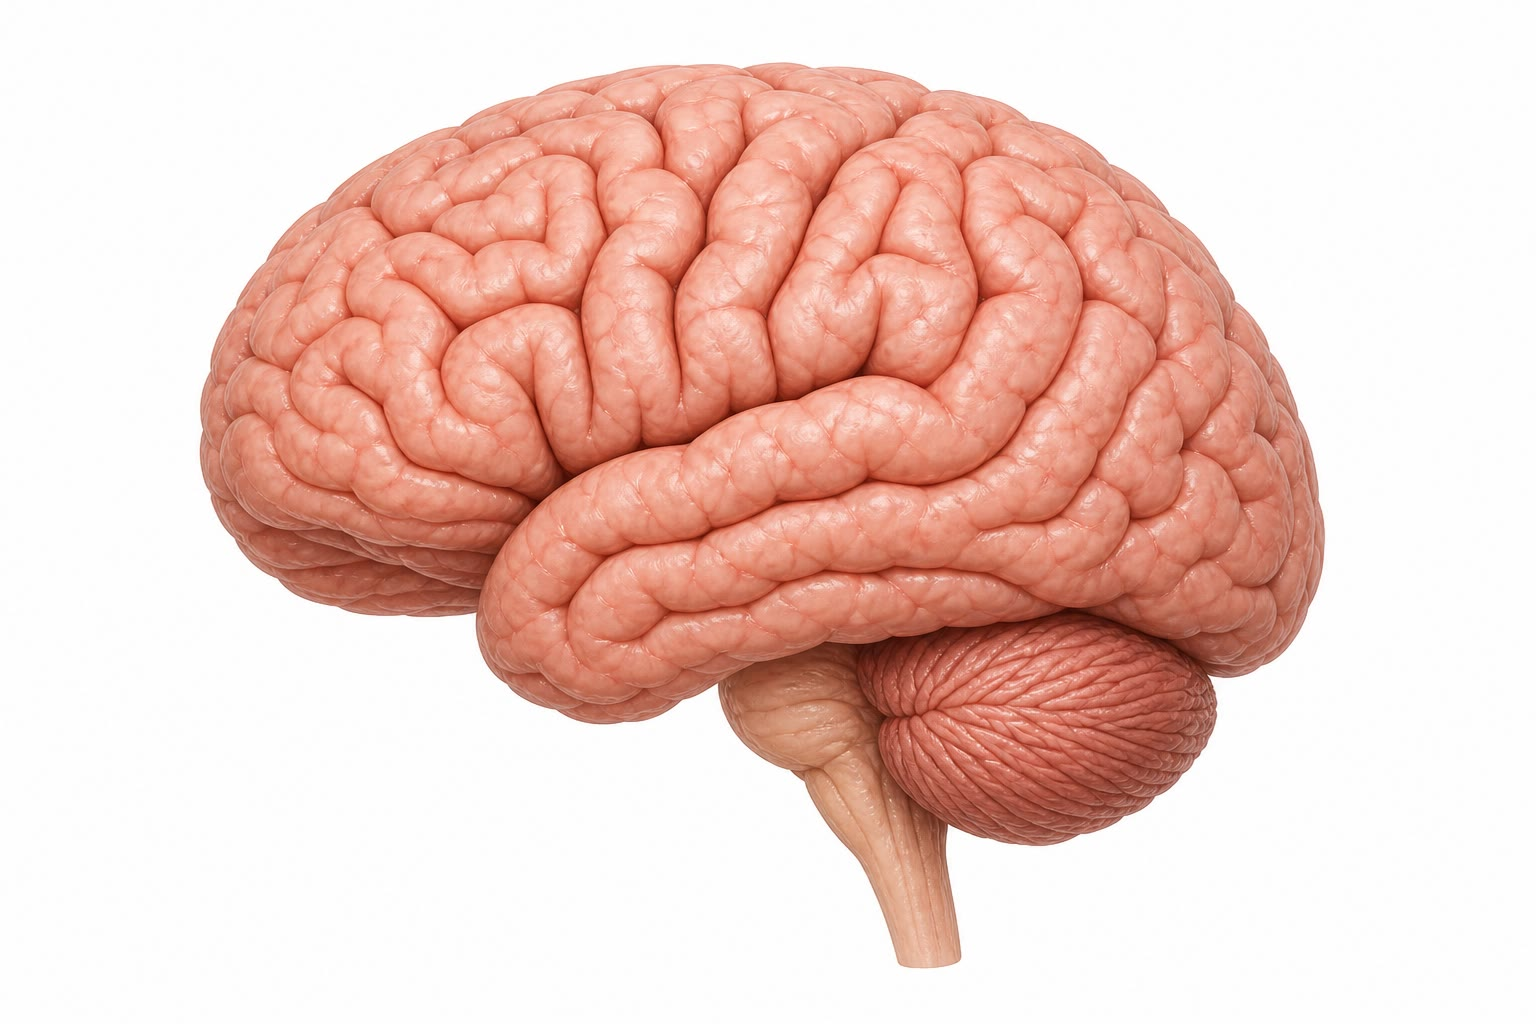
\includegraphics[width=0.52\linewidth]{images/book2/ai/fig-brain-side.jpg}};
  \begin{scope}[x={(img.south east)}, y={(img.north west)},
      every node/.style={font=\small}]
    \draw[omDef, thick] (0.85,0.55) -- (1.05,0.70) node[right, align=left] {初级视觉皮层 \\（枕叶）};
    \draw[omDef, thick] (0.70,0.75) -- (0.80,1.06) node[above] {顶叶};
    \draw[omDef, thick] (0.28,0.72) -- (0.20,1.06) node[above] {额叶};
    \draw[omDef, thick] (0.48,0.42) -- (0.40,-0.06) node[below] {颞叶};
    \draw[omDef, thick] (0.70,0.28) -- (1.05,0.20) node[right] {小脑};
  \end{scope}
\end{tikzpicture}

{\small 从左侧看大脑。\omterm{prop:g11:vision-and-brain:pathway}{初级视觉皮层}位于最后部，
即枕叶之中；更远的视觉区域从这里向前延伸，
进入颞叶（识别事物是什么）和顶叶
（定位事物在哪里以及如何运动）。}
\end{omfigure}

\section{多个区域，一种感知}

\begin{proposition}[专门化的视觉区域]\label{prop:g11:vision-and-brain:areas}
\omterm{prop:g11:vision-and-brain:pathway}{初级视觉皮层}将其分析交给十几个进一步的
\emph{视觉区域}，各有专门分工：一个提取颜色，一个负责
运动，其他的负责形状、深度、人脸和文字。它们的输出
与记忆、其他感觉相结合，汇合为
我们所体验到的单一而连贯的感知。感知是一种
构建：大脑填补盲点，补全隐藏的轮廓，
在光照变化时保持颜色恒定，并且会被
利用其规则的错觉所蒙骗。
\end{proposition}
\begin{proof}[证据]
局部损伤能将各个成分分离开来：颜色区域受损的患者
看到的世界是灰色的，但视力正常；运动区域受损时，
颜色和形状保持完好，却丧失了运动知觉；颞叶某一区域受损，
则仅使人脸识别能力丧失。
对健康志愿者进行功能成像显示，同样的区域会亮起：
一个区域对彩色图案有反应，另一个对运动的点有反应，
再一个对人脸有反应，而初级皮层对所有刺激都有反应。
动物实验中的电极记录发现，每个区域中的神经元只对该区域的
特征有反应，而几乎对其他刺激没有反应。
\end{proof}

\begin{omfigure}
\begin{tikzpicture}[font=\small, >=Stealth,
  b/.style={draw, rounded corners, align=center, text width=2.5cm, minimum height=1.0cm}]
  \node[b, fill=omDef!12] (ret) at (0,0) {视网膜：\\ 光转为信号};
  \node[b, fill=omDef!12] (v1) at (3.6,0) {初级视觉 \\ 皮层：边缘、\\ 方向、映射};
  \node[b, fill=omProp!15] (col) at (7.4,1.6) {颜色区域};
  \node[b, fill=omProp!15] (mov) at (7.4,0) {运动区域};
  \node[b, fill=omProp!15] (shp) at (7.4,-1.6) {形状与人脸 \\ 区域};
  \node[b, fill=omMeth!15, text width=2.8cm] (per) at (11.2,0) {感知：\\ 一个场景，\\ 并加入记忆};
  \draw[->, thick] (ret) -- (v1);
  \draw[->, thick] (v1) -- (col); \draw[->, thick] (v1) -- (mov); \draw[->, thick] (v1) -- (shp);
  \draw[->, thick] (col) -- (per); \draw[->, thick] (mov) -- (per); \draw[->, thick] (shp) -- (per);
\end{tikzpicture}

{\small 从信号到场景。初级皮层把其分析分配给
各专门区域，各区域的结果再重新整合。一个区域的损伤
去除一种属性——颜色、运动或人脸——而
其余部分保持完好。}
\end{omfigure}

\begin{example}[三位患者，三个区域]\label{ex:g11:vision-and-brain:patients}
看到世界是灰色的那位患者，双侧颜色区域受损；
她的视网膜\omterm{def:g11:the-eye:photoreceptors}{视锥细胞}工作正常，初级皮层也接收其
信号，但把\omterm{def:g11:the-eye:photoreceptors}{视锥细胞}比例转化为颜色的环节已经丧失。
看不见运动的患者丧失了运动区域，她看到的是
连续的静止画面。无法辨认人脸的患者，
颞叶的人脸区受损；她靠声音或帽子辨认
人。每种情况下，丧失的部分都很具体，而仍保留的
部分说明其他区域能够独立工作。
\end{example}

\section{由经验塑造的皮层}

\begin{proposition}[可塑性]\label{prop:g11:vision-and-brain:plasticity}
视觉皮层的连接在出生时并不固定。在
生命早期的\emph{关键期}内，这些连接由眼睛所见塑造；
成年后它们仍会继续变化，速度较慢，随学习和
使用而改变。这种\emph{大脑可塑性}\index{大脑可塑性}
是神经元的一种特性：被使用的连接会得到加强并增多，
未被使用的连接则会减弱并被修剪。
\end{proposition}
\begin{proof}[证据]
休伯尔与维泽尔（1960 年代）记录了猫和
猴的视觉皮层。正常动物中，多数神经元对两只眼睛都有反应。
若动物在出生后最初几个月中一只眼睛被闭合，
几乎所有神经元都只对睁开的眼睛有反应：闭合眼的
连接已被另一只眼睛占据。成年动物闭合一只眼睛相同
时间，却不会产生任何变化。人类中，若儿童一只眼睛
严重失焦或斜视，且在约 7 岁前未予矫正，
则会永久保留一只视力弱的眼——即弱视——
无论之后光学条件如何改善。成年人中，学习盲文会扩大
负责阅读手指的皮层区域；学习杂耍会扩大
处理运动信息的区域，若停止练习，这些区域又会
缩小。
\end{proof}

\begin{omfigure}
\begin{tikzpicture}
\begin{axis}[
  ybar, bar width=9pt,
  width=0.86\linewidth, height=5.6cm,
  axis x line=bottom, axis y line=left,
  ymin=0, ymax=60, ylabel={皮层神经元（\%）},
  ylabel style={font=\small},
   symbolic x coords={left eye only, mostly left, both equally, mostly right, right eye only},
  xtick=data, xticklabels={仅左眼, 以左眼为主, 两眼相当, 以右眼为主, 仅右眼}, tick label style={font=\small},
  xlabel={哪只眼睛驱动该神经元},
  xlabel style={font=\small, at={(axis description cs:0.5,-0.16)}, anchor=north},
  enlarge x limits=0.15, ytick={0,20,40,60},
  legend style={at={(0.5,-0.34)}, anchor=north, legend columns=2, font=\small, draw=none},
]
\addplot[fill=omDef!50, draw=omDef] coordinates  {(left eye only,12) (mostly left,20) (both equally,36) (mostly right,20) (right eye only,12)};
\addplot[fill=omThm!50, draw=omThm] coordinates  {(left eye only,2) (mostly left,3) (both equally,5) (mostly right,30) (right eye only,60)};
\legend{正常小猫, 左眼闭合三个月的小猫}
\end{axis}
\end{tikzpicture}

{\small 休伯尔与维泽尔的发现（取整）。正常小猫的大多数
视觉皮层神经元对两只眼睛都有反应。左眼闭合三个月后，
十个神经元中有九个只对右眼有反应：
未被使用的那只眼睛的连接已经消失。}
\end{omfigure}

\begin{example}[为何斜视必须及早治疗]\label{ex:g11:vision-and-brain:amblyopia}
3 岁儿童一只眼睛内斜，会看到重影，大脑
会抑制较弱的那个图像。若该眼未被矫正，或
健眼未每天遮挡数小时以迫使弱眼工作，
则在关键期内，皮层会围绕健眼重新组织，
弱眼虽然光学上完好，却
终身看不清精细细节。3 岁时治疗，儿童可恢复完全视力；
12 岁时治疗，几乎毫无效果。
\end{example}

\section{药物与视觉大脑}

\begin{proposition}[神经元、信使及模拟它们的分子]\label{prop:g11:vision-and-brain:drugs}
神经元在\emph{突触}处释放化学信使，
即\emph{神经递质}，作用于下一个
\omterm{def:g10:cells-common-unit:cell}{细胞}的受体；最后一年的课程将讲解其机制。若干种
神经递质，其中包括\emph{5-羟色胺}，共同调节
信号在视觉区域中的传递。形状与某种神经递质相似的分子
能够与其受体结合，扰乱这种传递：
麦角酸二乙基酰胺（LSD）与视觉皮层中的
5-羟色胺受体结合，产生幻觉——颜色、形状和
在无相应光照时所见的运动。此类药物可能留下
持久的改变：数月后仍会复发的发作，并在部分人身上
出现持续的视觉障碍。
\end{proposition}
\admitted

\begin{example}[幻觉说明了什么]\label{ex:g11:vision-and-brain:hallucination}
在 LSD 作用下，视网膜未变，\omterm{prop:g11:vision-and-brain:pathway}{初级视觉皮层}仍
对眼睛所见的内容加以映射；扰动出现在后续区域，以及
它们的组合方式上。出现的图案类似皮层自身的
构件——网格、螺旋、隧道——这是因为药物
使感知机制在没有输入的情况下运转。
幻觉以失效的方式表明：看见是由大脑完成的，
而一种分子能够改变它。
\end{example}

\begin{method}[定位视觉缺陷]\label{met:g11:vision-and-brain:locate}
\begin{enumerate}
  \item 一只眼失明，另一只正常：眼睛或其视神经，
        位于视交叉之前。
  \item 双眼在视野的同一半失明：对侧的
        视束、丘脑或\omterm{prop:g11:vision-and-brain:pathway}{初级视觉皮层}。
  \item 双眼在视野外侧一半失明：视交叉，
        即交叉纤维被切断之处。
  \item 视觉完好，但某一特征丧失（颜色、运动、面孔）：
        相应的特化区域。
  \item 眼睛和皮层均正常，但感知受干扰，属暂态：一种
        药物或\omterm{def:g10:cell-metabolism:metabolism}{代谢}原因。
\end{enumerate}
\end{method}

\begin{remark}[本年的收获]\label{rem:g11:vision-and-brain:year}
在\cref{ch:g11:the-eye}中，眼睛是\omterm{def:g10:universal-dna:gene}{基因}与\omterm{def:g11:gene-expression:protein}{蛋白质}的问题：
\omterm{def:g11:the-eye:photoreceptors}{视蛋白}、它们的重复，以及 X \omterm{def:g11:cell-cycle-mitosis:chromosome}{染色体}遗传的色盲。
本章的大脑则是连接的问题，由使用塑造。
二者之间，是本年的全部内容——从\omterm{def:g10:universal-dna:gene}{基因}的序列
到性状，再从性状到一个人能做什么——
以及这一道理：每一步中，\omterm{def:g11:enzymes-and-phenotype:phenotype}{基因型}提出可能，而
环境（从猫耳朵的温度到小猫眼睛接收到的光）
则作出安排。
\end{remark}

\section{练习}

\begin{exercise}[$\star$]\label{exo:g11:vision-and-brain:1}
追踪信号从视野左半侧到
皮层的传递路径。
\end{exercise}

\begin{exercise}[$\star$]\label{exo:g11:vision-and-brain:2}
视交叉处发生了什么？哪些纤维发生交叉？
\end{exercise}

\begin{exercise}[$\star$]\label{exo:g11:vision-and-brain:3}
说出三个视觉特化区域，以及
每一区域受损所导致的缺陷。
\end{exercise}

\begin{exercise}[$\star$]\label{exo:g11:vision-and-brain:4}
给出\omterm{prop:g11:vision-and-brain:plasticity}{大脑可塑性}和关键期的定义。
\end{exercise}

\begin{exercise}[$\star$]\label{exo:g11:vision-and-brain:5}
LSD 如何作用于视觉系统？
\end{exercise}

\begin{exercise}[$\star\star$]\label{exo:g11:vision-and-brain:6}
利用\cref{met:g11:vision-and-brain:locate}，定位
一名双眼视野右半侧失明患者的损伤部位。
\end{exercise}

\begin{exercise}[$\star\star$]\label{exo:g11:vision-and-brain:7}
一个\omterm{def:g11:cancer:cancer}{肿瘤}从下方压迫视交叉，切断交叉的
纤维。患者丧失了视野的哪些部分？请结合
图示说明。
\end{exercise}

\begin{exercise}[$\star\star$]\label{exo:g11:vision-and-brain:8}
根据休伯尔–维泽尔图，在正常小猫和被剥夺的小猫中，
分别有多大比例的神经元对左眼有任何反应？
\end{exercise}

\begin{exercise}[$\star\star$]\label{exo:g11:vision-and-brain:9}
为何让斜视儿童的好眼每天遮住几个小时，
就能治疗弱视？同样的治疗为何对成人无效？
\end{exercise}

\begin{exercise}[$\star\star$]\label{exo:g11:vision-and-brain:10}
解释为何只能看到灰色的患者，按
\cref{ch:g11:the-eye}中的含义并不属于色盲，
并说明怎样的检测能够区分这两种情况。
\end{exercise}

\begin{exercise}[$\star\star$]\label{exo:g11:vision-and-brain:11}
一位钢琴家负责手指的皮层区域比平均水平更大。
用可塑性加以解释，并说明若她
停止弹琴多年，你预测会发生什么。
\end{exercise}

\begin{exercise}[$\star\star\star$]\label{exo:g11:vision-and-brain:12}
一名因白内障而生来失明的人，三十岁时接受手术摘除白内障。
请预测她最初几周会看到什么，以及哪些能够
恢复、哪些不能恢复，并利用关键期加以说明。
\end{exercise}

\begin{exercise}[$\star\star\star$]\label{exo:g11:vision-and-brain:13}
解释为何皮层映射图为视野中央
分配的面积多于周边，并利用\cref{ch:g11:the-eye}中
感受器与神经节\omterm{def:g10:cells-common-unit:cell}{细胞}的分布加以说明。
\end{exercise}

\begin{exercise}[$\star\star\star$]\label{exo:g11:vision-and-brain:14}
功能成像显示，受试者闭眼
想象一个红苹果时，颜色区域处于活跃状态。这说明了
特化区域与感知之间的关系，以及关于
幻觉的哪些结论？
\end{exercise}

\begin{exercise}[$\star\star\star$]\label{exo:g11:vision-and-brain:15}
“看见是由眼睛完成的。”请正确改写这一说法，
写成一段话，并运用三位患者、小猫和药物的例子。
\end{exercise}

\section{问题：四名患者与一只小猫}

\begin{problem}[{周末问题——沿通路定位的视觉缺损，由刺激绘制的皮层，
对小猫视觉剥夺的计量，
以及及时治疗儿童斜视}]
\label{pb:g11:vision-and-brain:1}
四名患者接受检查。A：左眼失明，右眼
正常。B：两眼均对视野左半侧失明。C：两眼均
对各自视野的外侧一半失明（左眼为左侧，右眼
为右侧）。D：视野正常，视力正常，但
无法感知运动。

\medskip
\noindent\textbf{第一部分——定位。}
\begin{enumerate}
  \item 定位 A 的损伤，指出是哪一结构，以及它位于视交叉
        之前还是之后？
  \item 定位 B 的损伤，并说明它为何必须位于视交叉之后。
  \item 精确定位 C 的损伤，并说明哪些纤维被切断。
  \item 定位 D 的损伤。视野和视力得以保留，
        这说明了\omterm{prop:g11:vision-and-brain:pathway}{初级视觉皮层}的什么特点？
  \item 对每名患者，判断视网膜是否完好，
        并说明你会如何检查。
\end{enumerate}

\medskip
\noindent\textbf{第二部分——皮层映射图。}
手术中，刺激患者右侧视皮层的若干点，
会产生闪光。刺激枕叶尖端，得到的闪光位于视野中央；
刺激更靠前的点，闪光则出现在左侧视野中更外侧的位置；
皮层尖端每 \qty{1}{cm} 覆盖视野
约 $2^\circ$，而向前 \qty{1}{cm} 覆盖
$20^\circ$。
\begin{enumerate}[resume]
  \item 为什么所有闪光都位于左侧视野？
  \item 表示中央 $2^\circ$ 的皮层，与
        $2^\circ$ 宽、位于距中心 $40^\circ$ 处的条带相比，有多大？计算其比值。
  \item 将此比值与视网膜的中央凹和周边部加以联系。
  \item 右侧枕叶尖端出现小损伤时，患者会失去什么？
        若同样大小的损伤位于更靠前处，
        患者又会失去什么？
  \item 为什么中央区域有小损伤的患者，仍能
        通过转动眼睛缓慢阅读？
\end{enumerate}

\medskip
\noindent\textbf{第三部分——小猫。}
依据休伯尔–维泽尔图。
\begin{enumerate}[resume]
  \item 正常小猫中，有多大百分比的神经元
        对两眼都有一定程度的反应？
  \item 在被剥夺视觉的小猫中，有多大百分比的神经元
        对闭合的（左）眼是否还有反应？
  \item 闭合眼的视网膜和视神经均完好，其输入信号
        去了哪里？又是什么占据了其空间？
  \item 同样的闭合作用于成年猫时，毫无改变。这
        说明了什么？其人类对应的情形是什么？
  \item 一只小猫双眼闭合三个月。预测其
        直方图，以及此后该动物的视力。
\end{enumerate}

\medskip
\noindent\textbf{第四部分——儿童。}
一名四岁儿童的左眼向内偏斜，其光学系统正常。
若不治疗，皮层会接管右眼的输入信号。
\begin{enumerate}[resume]
  \item 结合小猫的例子，解释若不加处理，左眼的视觉
        会发生什么变化，以及为何仅靠眼镜无法
        防止这种情况发生。
  \item 治疗方法是每天遮盖\emph{右眼}数小时，
        持续数月。解释为何遮盖的是健康的那只眼。
  \item 为何这一治疗必须在七岁左右之前进行，又为何
        同样的治疗在十五岁时会失效？
  \item 三十岁时失去一只眼的成年人，其为该眼
        服务的皮层并不以同样方式丧失。请将此与小猫的结果统一解释。
  \item 请陈述结论：沿通路从前向后定位的四处损伤，
        以及皮层中需要指明名称的那一性质——
        它使儿童的治疗只有及时进行才会奏效。
\end{enumerate}
\end{problem}
